% !TEX root = main.tex
\documentclass[../main.tex]{subfiles}
\begin{document}

\section{Stability of fluid flows}
\label{sec:stability}

Let us investigate the following PDE:
\[
	\begin{cases}
		\partial_t u = \partial_{xx}u + au, & \, \text{in} \, \Omega = (0,1) \\
		u(t,x) = 0, & \, \text{on} \, x=0, x=1
	\end{cases}.
\]
Clearly, $\hat{u}(t,x) = 0$ is a solution, moreover it is a \textit{steady solution}. Our interest is whether, given some initial condition $u_0(x)$the solution converges to the steady one; in other words, whether
\[
	" \lim_{t \to \infty}u(t,x) = 0",
\]
in some sense of convergence. 


\subsection{Energy theory}
\label{sec:energy_theory}
One way would be to linearize and then deploy some linearized stability analysis techniques (as in the case of ODE's). However, we do not want to lose any information (\textit{i.e.}, any phenomena) described by the full system; a different technique is needed. Let us measure the convergence in the $\LpSet[2]{\Omega}$ norm, "the energy norm", \textit{i.e.}
\[
	\norm{u}_{\LpSet[2]{\Omega}} = \qty(\int_{\Omega}|u|^{2}\dd{x})^{\frac{1}{2}}.
\]
Meaning we are interested in the conditions under which
\[
	u \to 0 \, \text{in} \,\LpSet[2]{\Omega} \Leftrightarrow \norm{u}_{\LpSet[2]{\Omega}} \to 0.
\]
Let us investigate the following quantity:
\begin{align*}
	\frac{1}{2}\dv{t} \norm{u}_{\LpSet[2]{\Omega}}^{2} &= \frac{1}{2} \dv{t} \int_{\Omega}u\qty(t,x) u\qty(t,x)\dd{x} = \int_{\Omega}\partial_t u\qty(t,x) u\qty(t,x)\dd{x} =\\
							   &=\int_{\Omega}\qty(u \partial_{xx}u+ a u^{2})\dd{x} = -\int_{\Omega}\qty(\partial_x u)^{2}\dd{x} + a \int_{\Omega}u^{2}\dd{x} = \\
							   & = -\norm{\partial_x u}_{\LpSet[2]{\Omega}}^{2} + a \norm{u}_{\LpSet[2]{\Omega}}^{2} \leq - \frac{1}{C_p^{2}}\norm{u}_{\LpSet[2]{\Omega}}^{2}+a \norm{u}_{\LpSet[2]{\Omega}}^{2} =\\
							   &=-\qty(\frac{1}{C_p^{2}}-a)\norm{u}_{\LpSet[2]{\Omega}}^{2},
\end{align*}
where we used the Poincare inequality in the form $\norm{u}_{\LpSet[2]{\Omega}} \leq C_p \norm{\partial_x u}_{\LpSet[2]{\Omega}}$ (we have zero trace). So we have :
\[
	\dv{t} \norm{u}_{\LpSet[2]{\Omega}}^{2} \leq -2\qty(\frac{1}{C_p^{2}}-a)\norm{u}_{\LpSet[2]{\Omega}}^{2},
\]
so if
\[
	\frac{1}{C_p^{2}}-a>0,
\]
the norm satisfies the following differential inequality

\[
	\norm{u}_{\LpSet[2]{\Omega}}\leq \exp\qty(-t\sqrt{\frac{1}{C_p^{2}}-a})\norm{u_0}_{\LpSet[2]{\Omega}},
\]
and so
\[
	\norm{u(t,x)}_{\LpSet[2]{\Omega}} \to 0, \, \text{as} \, t\to \infty.
\]
We are not happy yet. The Poincare constant is undetermined, so let us get an estimate for it. The equation has the form
\begin{align*}
	\frac{1}{2}\dv{t} \norm{u}_{\LpSet[2]{\Omega}}^{2} &= - \norm{\partial_x u}_{\LpSet[2]{\Omega}}^{2}+a \norm{u}_{\LpSet[2]{\Omega}}^{2} = -a \norm{\partial_x u}_{\LpSet[2]{\Omega}}^{2}\qty(\frac{1}{a}-\frac{\norm{u}_{\LpSet[2]{\Omega}}^{2}}{\norm{\partial_x u}_{\LpSet[2]{\Omega}}^{2}}) \leq \\
	&\leq -a \norm{\partial_x u}_{\LpSet[2]{\Omega}}^{2}\qty(\frac{1}{a}-\max_{u \in \WkpzeroSet[1][2]{\Omega}}\frac{\norm{u}_{\LpSet[2]{\Omega}}^{2}}{\norm{\partial_x u}_{\LpSet[2]{\Omega}}}),
\end{align*}
let us define
\[
	\frac{1}{a_{\, \text{crit} \,}} = \max_{u \in \WkpzeroSet[1][2]{\Omega}}\frac{\norm{u}_{\LpSet[2]{\Omega}}^{2}}{\norm{\partial_x u}_{\LpSet[2]{\Omega}}^{2}},
\]
and so we have
\[
	\frac{1}{2}\dv{t}\norm{u}_{\LpSet[2]{\Omega}}^{2} \leq -a \norm{\partial_x u}_{\LpSet[2]{\Omega}}^{2}\qty(\frac{1}{a}-\frac{1}{a_{\, \text{crit} \,}}) = -a \norm{\partial_x u}_{\LpSet[2]{\Omega}}^{2} \frac{a_{\, \text{crit} \,}-a}{a a_{\, \text{crit} \,}}.
\]
We see that if $a < a_{\, \text{crit} \,} \Leftrightarrow \frac{1}{a} > \frac{1}{a_{\, \text{crit} \,}}$ the $\LpSet[2]{\Omega}$ norm vanishes exponentially.
But \textit{how much is it?} That depends on $a_{\, \text{crit} \,},$ so let us define the functional
\[
	F: \WkpzeroSet[1][2]{\Omega} \to \R^+, F: u \mapsto \frac{\norm{u}_{\LpSet[2]{\Omega}}^{2}}{\norm{\partial_x u}_{\LpSet[2]{\Omega}}^{2}},
\]
and find its extrema. The Gateux derivative at the extrema is
\begin{align*}
	0 = &\delta F\qty(u_{\, \text{ext} \,})[v] = \dv{t} \eval{F\qty(u_{\, \text{ext} \,} + t v)}_{t=0} = \dv{t} \eval{\frac{\int_{\Omega}\qty(u_{\, \text{ext} \,}+tv)\qty(u_{\, \text{ext} \,}+tv)\dd{x}}{\int_{\Omega}\qty(\partial_x u_{\, \text{ext} \,}+t \partial_x v)\qty(\partial_x u_{\, \text{ext} \,}+t \partial_xv)\dd{x}}}_{t=0} =\\
	    & = 2\frac{\int_{\Omega}u_{\, \text{ext} \,}v\dd{x}\int_{\Omega}\qty(\partial_x u_{\, \text{ext} \,})^{2}\dd{x} - \int_{\Omega}u_{\, \text{ext} \,}^{2}\dd{x}\int_{\Omega}\partial_x u_{\, \text{ext} \,} \partial_x v\dd{x}}{\qty(\int_{\Omega}\qty(\partial_x u_{\text{ext}})^{2}\dd{x})^{2}} = \\
	    & = \frac{1}{\qty(\int_{\Omega}\qty(\partial_x u_{\, \text{ext} \,})^{2}\dd{x})^{2}}\qty(\int_{\Omega}u_{\, \text{ext} \,}v\dd{x}-\frac{\int_{\Omega}u_{\, \text{ext} \,}^{2}\dd{x}}{\int_{\Omega}\qty(\partial_x u_{\text{ext}})^{2}\dd{x}} \int_{\Omega}\partial_x u_{\, \text{ext} \,} \partial_x v\dd{x}) =\\
	    &=\frac{1}{\int_{\Omega} (\partial_x u_{\, \text{ext} \,})^{2}\dd{x}} \frac{1}{a_{\, \text{crit} \,}}\qty(\int_{\Omega}\qty(a_{\, \text{crit} \,}u_{\, \text{ext} \,}v - \partial_x u_{\, \text{ext} \,}\partial_x v)\dd{x}),
\end{align*}
and so we see
\[
	\delta F\qty(u_{\, \text{ext} \,})[v] = 0 \Leftrightarrow \int_{\Omega}\qty(a_{\, \text{crit} \,} u_{\, \text{ext} \,} v - \partial_x u_{\, \text{ext} \,} \partial_x v)\dd{x} = 0, 
\]
This is a weak formulation of the problem
\[
	\int_{\Omega}\qty(a_{\, \text{crit} \,} u_{\, \text{ext} \,}+ \partial_{xx}u_{\, \text{ext} \,})v\dd{x}, \forall v \in \WkpzeroSet[1][2]{\Omega} \Leftrightarrow \begin{cases}\partial_{xx}u_{\, \text{ext} \,} =  a_{\, \text{crit} \,}u_{\, \text{ext} \,}, & \, \text{in} \,\Omega \\
		u_{\, \text{ext} \,} = 0,& \, \text{on} \, \partial \Omega 
	\end{cases}.
	\]
	This is an \textit{eigenproblem for the elliptic operator} (from the original parabolic operator). The solution is the following:
	\begin{align*}
		u_{\, \text{ext} \,}^n &= C \sin\qty(\sqrt{a_{\, \text{crit} \,}^n}x), \\
		a^n_{\, \text{crit} \,} &= n^{2}\pi^{2}, n \in \N
	\end{align*}
The \textit{smallest eigenvalue} is
\[
	a_{\, \text{crit} \,} = \pi^{2}.
\]
This means that
\[
	\forall a < a_{\, \text{crit} \,} = \pi^{2},
\]
the perturbations in the initial condition decay exponentially.

\subsection{Rayleigh-Bénard convection}
\label{sec:convection}
Let us use the developed theory on the problem of Rayleigh-Bénard convection. 

\begin{center}
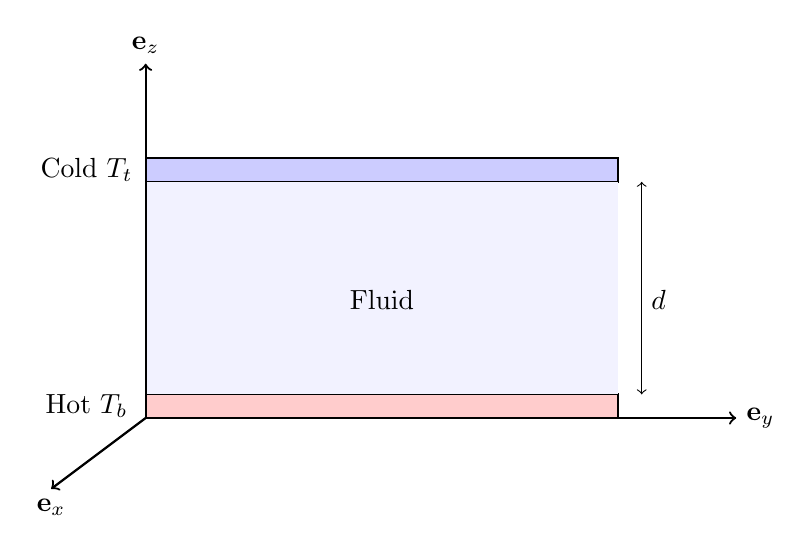
\begin{tikzpicture}[scale=1.5]

  % Coordinates
  \def\width{4}  % Width of the plates in y
  \def\depth{2}  % Not shown (x-direction into the page)
  \def\d{2}      % Distance between plates (z-direction)

  % Draw bottom plate
  \draw[thick, fill=red!20] (0, 0) rectangle (\width, 0.2);
  \node at (-0.5, 0.1) {Hot $T_b$};

  % Draw top plate
  \draw[thick, fill=blue!20] (0, \d) rectangle (\width, \d + 0.2);
  \node at (-0.5, \d + 0.1) {Cold $T_t$};

  % Draw fluid region
  \fill[blue!5] (0, 0.2) rectangle (\width, \d);
  \node at (\width/2, \d/2) {Fluid};

  % Dimension d
  \draw[<->] (\width + 0.2, 0.2) -- (\width + 0.2, \d);
  \node[right] at (\width + 0.2, \d/2) {$d$};

  % Axes
  \draw[->, thick] (0, 0) -- (0, \d + 1) node[above] {$\mathbf{e}_z$};
  \draw[->, thick] (0, 0) -- (\width + 1, 0) node[right] {$\mathbf{e}_y$};
  \draw[->, thick] (0, 0) -- (-0.8, -0.6) node[below] {$\mathbf{e}_x$};
.

\end{tikzpicture}
\end{center}

There are two parallel infinite plates, the top with the temperature $T_t$ and the bottom one with the temperature $T_b$ in the gravitational field $\vb{g}= - g \vb{e}_z.$ The space is filled with a compressible Navier Stokes fluid, so the governing equations are
\begin{align*}
	\dv{\rho}{t} + \rho \qty(\divergence{\vb{v}}) &= 0, \\
	\rho \dv{\vb{v}}{t} &= \rho \vb{g} + \divergence{\qty(-\pth\qty(\rho, \theta)\identity + \lambda \qty(\divergence{\vb{v}})\identity + 2 \mu \symvgrad)} \\
	\rho c_{V}\dv{\theta}{t} &= \divergence{\qty(\kappa \grad \theta)}+\qty(\pth\qty(\theta, \rho)-\pdv{\pth\qty(\theta, \rho)}{\theta})\qty(\divergence{\vb{v}}) + \cstress : \symvgrad,
\end{align*}
Why is anything happening at all?
\begin{itemize}
	\item gravitational field is crucial, as without it, buyoancy oscillations won't work
	\item dependence of density on temperature is also essential
\end{itemize}

\subsubsection{Boussinesq-Oberbeck approximation}
\label{sec:boussinesq_approximation}
Doing a stability analysis of a system of nonlinear PDEs is difficult. We adopt the following assumptions, known as the \textit{Oberbeck-Boussinesq approximation}

\begin{itemize}
	\item the density depends only on the temperature, not on pressure, and only linearly: $\rho(\theta) = \rho_{\, \text{ref} \,}\qty(1- \alpha\qty(\theta - \theta_{\, \text{ref} \,}))$
	\item working with compressible fluids is a nightmare, lets make it incompressible: $\divergence{\vb{v}} = 0.$
	\item the density in the momentum equation is constant in the first term and the same in the temperature equation
	\item ignore all the nonlinear terms in the thermal equation
\end{itemize}
Doing all this produces the following system of equations:
\begin{align}
	\label{eq:ober_boussinesq}
	\divergence{\vb{v}} &= 0, \\
	\rho_{\, \text{ref} \,} \dv{\vb{v}}{t} &= \rho_{\, \text{ref} \,}\qty(1- \alpha\qty(\theta-\theta_{\, \text{ref} \,})) \vb{g} + \divergence{\qty(-\pth\qty(\rho, \theta)\identity +  2 \mu \symvgrad)} \\
	\rho_{\, \text{ref} \,} c_{V}\dv{\theta}{t} &= \divergence{\qty(\kappa \grad \theta)},
\end{align}
with the boundary conditions
\[
	\begin{cases}
		\theta &=T_{t}, \, \text{on} \, \qty{z=d} \\
		\theta &=T_{b}, \, \text{on} \,\qty{z=0}
	\end{cases}
\]

Note that, physically, this \textit{approximation makes no sense}. Since $\cstress : \symvgrad = 0$, there is no viscous dissipation, but also $\cstress \neq \tensorq{0}$, so we are just losing energy but the temperature does not increase. Nevertheless, this approximation is popular and often used.

\subsubsection{Steady state, pure conduction}
\label{sec:steady_state}

With the system of our interest \ref{eq:ober_boussinesq} defined, let us investigate the stability of the steady state. What does it look like?

Clearly, the simplest case would be
\[
	\vb{\hat{v}} = \vb{0},
\]
and the remaning qualities need to solve the stationary versions of the present equations; the equation for the temperature reads 
\[
	0 = \divergence{\qty(\kappa \grad \hat{\theta})},
\]
with the solution 
\begin{equation}
	\label{eq:steady_temp}
	\hat{\theta} = \hat{\theta}(z) = - \frac{T_{b}-T_{t}}{d}z + T_{bot} = -\beta z + T_{bot},
\end{equation}
where we have denoted
\[
	\beta = \frac{T_b - T_t}{d},
\]
as the temperature gradient.
The pressure has to solve the rest of the momentum equation, that is
\[
	0 = - \grad \hat{p} - \rho_{\, \text{ref} \,}\qty(1-\alpha\qty(\theta(z) - \theta_{\, \text{ref} \,}))g \vb{e}_{z},
\]
which has the solution
\[
	\hat{p}(z) = -\rho_{\, \text{ref} \,}g \int_0^z \qty(1-\alpha\qty(\theta(s)-\theta_{\, \text{ref} \,}))\dd{s}.
\]
The triple $\qty(\hat{\vb{v}}, \hat{\theta}, \hat{p})$ will be our steady solution from now on.

\subsubsection{Perturbation of the steady state, convection}
\label{sec:perturbation}
What happens if now perturb the steady state? We are solving the following system
\[
	\begin{cases}
		\divergence{\vb{v}} = 0, \\
		\rho_{\, \text{ref} \,}\qty(\partial_t \vb{v}+ \qty(\vb{v} \vdot \grad)\vb{v}) = -\rho_{\, \text{ref} \,}\qty(1- \alpha\qty(\theta-\theta_{\, \text{ref} \,}))g \vb{e}_z - \grad p + \mu \laplace \vb{v}\\ 
		\rho_{\, \text{ref} \,} c_{V}\qty(\partial_t \theta + \qty(\vb{v} \vdot \grad)\theta) = \kappa \laplace\theta
	\end{cases},
\]
with the initial conditions given as
\[
	\vb{v} = \hat{\vb{v}} + \tilde{\vb{v}} = \tilde{\vb{v}}, \theta = \hat{\theta}+ \tilde{\theta}, p = \hat{p}+ \tilde{p}
\]
all at $t =0$. The the hatted variables are the steady state, the tildas are perturbations. Incompressibility yields

\[
	\divergence{\qty(\vb{\hat{v}}+ \vb{\tilde{v}})} = 0 = \divergence{\vb{\tilde{\vb{v}}}},
\]
because $\vb{\hat{\vb{v}}} = \vb{0}.$ The momentum equation is

\[
	\rho_{\text{ref}}\qty(\partial_t \tilde{\vb{v}} + \qty(\vb{\tilde{v}}\vdot \grad)\vb{\tilde{v}}) = -\rho_{\text{ref}}\qty(1- \alpha\qty(\hat{\theta} + \tilde{\theta} - \theta_{\text{ref}}))g \vb{e}_z - \grad \qty(\hat{p}+ \tilde{p}) + \mu \laplace \vb{\tilde{v}},
\]
so upon plugging in $\grad \hat{p} = - \rho_{\text{ref}}\qty(1 - \alpha\qty(\hat{\theta}- \theta_{\text{ref}}))g \vb{e}_z,$ the equation becomes
\[
	\rho_{\text{ref}}\qty(\partial_t \vb{\tilde{\vb{v}}}+ \qty(\vb{\tilde{v}}\vdot \grad)\vb{\tilde{v}}) = \rho_{\text{ref}} \alpha g \vb{e}_z \tilde{\theta} - \grad \tilde{p} + \mu \laplace \vb{\tilde{v}},
\]
and finally, the heat equation is
\[
	\rho_{\text{ref}} c_V\qty(\partial_t \hat{\theta} + \partial_t \tilde{\theta} + \qty(\vb{\tilde{v}}\vdot \grad)\qty(\hat{\theta}+ \tilde{\theta}))= \kappa \laplace\qty(\hat{\theta} + \tilde{\theta}),
\]
so upon using the fact $\partial_t \hat{\theta} = 0, \laplace \hat{\theta} = 0,$ we obtain
\[
	\rho_{\text{ref}} c_V\qty(\partial_t \hat{\theta} + \qty(\vb{\tilde{v}} \vdot \grad)\qty(\hat{\theta}+ \tilde{\theta})) = \kappa \laplace \tilde{\theta}.
\]
Altogether, the perturbation $\qty(\tilde{\vb{v}}, \tilde{\theta}, \tilde{p})$ solves the following system

\begin{align}
	\label{eq:system_perturbations}
	\divergence{\tilde{\vb{v}}} &= 0, \\
	\rho_{\, \text{ref} \,}\qty(\partial_t \tilde{\vb{v}}+ \qty(\tilde{\vb{v}} \vdot \grad)\tilde{\vb{v}}) &= +\rho_{\, \text{ref} \,} \alpha g \vb{e}_z \tilde{\theta} - \grad \tilde{p} + \mu \laplace \tilde{\vb{v}}\\ 
\rho_{\, \text{ref} \,} c_{V}\qty(\partial_t \tilde{\theta} + \qty(\tilde{\vb{v}} \vdot \grad)\qty(\hat{\theta} + \tilde{\theta})) &= \kappa \laplace\tilde{\theta}.
\end{align}


\subsubsection{Non-dimensonalisation}
\label{sec:dimless}
We seek some quality that would characterize the stability of the flow. It would be most convenient for this quantity to be dimensionless, accounting for all the geometry, choice of units and other things. For that, let us choose 
\begin{itemize}
	\item a characteristic length: $l_{\text{char}} \coloneq d$
	\item a characteristic density $\rho_{\text{char}} \coloneq  \rho_{\, \text{ref} \,}$
	\item a characteristic temperature $\theta_{\text{char}} = T_{b}-T_{t}$
	\item a characteristic time $t_{\text{char}} = ?$
\end{itemize}
There is however a problem: \textit{how to choose the characteristic time?} We have no characteristic velocity \footnote{If we would, that would suffice, as we have characteristic length.}, because
\[
	\hat{\vb{v}} = \vb{0}.
\]
There are some candidates whose units include seconds:
\[
	[\mu] = \unit{Pa \cdot s}, [g] = \unitfrac{m}{s^{2}}, [\kappa] = \unitfrac{W}{m \cdot K},
\]
so we can in theory choose one and using that define $t_{\text{char}}.$ Let us continue: with the characteristic time being chosen, we can also set the characteristic velocity as
\[
	v_{\text{char}} = \frac{l_{\text{char}}}{t_{\text{char}}}.
\]
so we can rewrite the qualities \footnote{
	\[
		\unit{Pa} = \unitfrac{N}{m} = \unitfrac{kg \cdot m}{s^{2} m^{2}} = \unitfrac{\unitfrac{kg}{m^{3}} m^{3}}{s^{2} m} = \unitfrac{\unitfrac{kg}{m^{3}} m^{2}}{s^{2}}
	\]
}
\[
	\vb{\tilde{v}} = v_{\text{char}} \vb{v^{*}}, t = t_{\text{char}} t^{*}, \vb{x} = l_{\text{char}} \vb{x^{*}}, \tilde{\theta} = \theta_{\text{char}} \theta^{*}, \tilde{p} = \frac{\rho_{\text{ref}} l_{\text{char}}^{2}}{t_{\text{char}}^{2}} p^{*}
\]
Plugging this into the equations for the perturbation \ref{eq:system_perturbations} and denoting (for the time being) the dimensionless variables with stars, we obtian

\begin{align*}
		\grad^{*} \vdot \vb{v}^{*} &= 0 \\
		\frac{\rho_{\text{ref}}d^{2}}{\mu t_{\text{char}}}\qty(\partial_{t^{*}} \vb{v}^{*} + \qty(\vb{v}^{*} \vdot \grad^{*})\vb{v}^{*}) &= - \grad^{*} p^{*} + \laplace^{*} \vb{v}^{*} + \frac{\alpha g \theta_{\text{char}}d \rho_{\text{ref}} t_{\text{char}}}{\mu}\theta^{*} \vb{e}_z\\
		\partial_{t^{*}}\theta^{*} + \qty(\vb{v}^{*} \vdot \grad^{*})\theta^{*}&= \divergence{\qty(\frac{\kappa t_{\text{char}}}{\rho_{\text{ref}}c_V d^{2}}\grad^{*} \theta^{*})}- v^{*}_z,
\end{align*}
where we have denoted
\[
	v^{*}_z = \rho_{\text{ref}} c_V \tilde{\vb{v}}\vdot \grad \hat{\theta} = \rho_{\text{ref}} c_V \tilde{\vb{v}} \vdot \grad \qty(\frac{-\theta_{\text{char}}}{d}z + T_{b}) =- \rho_{\text{ref}} c_V \frac{\theta_{\text{char}}}{d}\vb{e}_z \vdot \vb{\tilde{v}}
\]

And now we see how the choice of $t_{char}$ influences the equations. I can require one of the following
\begin{align*}
		\frac{\rho_{\text{ref}}d^{2}}{\mu t_{\text{char}}} &= 1,\\
		\frac{\alpha g \theta_{\text{char}}d \rho_{\text{ref}}t_{\text{char}}}{\mu} &= 1,\\
		\frac{\kappa t_{\text{char}}}{\rho_{\text{ref}}c_Vd^{2}} &=1.
\end{align*}
Each of these choices are sensible. In our case, we are interested in the thermal conduction mainly, so let us choose
\[
	t_{\text{char}} = \frac{\rho_{\text{ref}}c_V d^{2}}{\kappa}.
\]
Finally, we arrive to the following system of equations (we omit the stars and tildas)
\begin{align*}
	\divergence{\vb{v}} &= 0, \\
	\frac{1}{\, \text{Pr} \,}\qty(\partial_t \vb{v}+\qty(\vb{v} \vdot \grad)\vb{v}) &= - \grad p + \laplace \vb{v} + \, \text{Ra} \,\theta \vb{e}_z, \\
	\partial_t \theta + \qty(\vb{v} \vdot \grad)\theta &=  \laplace \theta + v_z,
\end{align*}
where
\begin{equation}
\label{eq:prandtl_number}
	\, \text{Pr} \, = \frac{\nu}{k} = \frac{\rho_{\text{ref}} d^{2}}{\mu t_{\text{char}}},
\end{equation}
is the Prandtl number and
\begin{equation}
\label{eq:rayleigh_number}
	\, \text{Ra} \, = \frac{\alpha g \theta_{\text{char}}d^{3}}{\nu k}, \nu = \frac{\mu}{\rho_{\text{ref}}}, k = \frac{\kappa}{\rho_{\text{ref}}c_V}.
\end{equation}
is the Rayleigh number.


Another form of the equations can be derived when rescaling the temperateure (choosing a different characteristic temperature)\footnote{Of course $\theta^{*}$ is totally different than the previous one}
\begin{equation}
	\label{eq:another_temp_scaling}
	\theta = \frac{\, \text{Pr} \,}{\sqrt{\, \text{Ra} \,}}\theta^{*},
\end{equation}
and this leads (of course, other quantities will have to be rescaled as well)

\begin{align*}
	 \grad^{*} \vdot \vb{v}^{*}&= 0 \\
	\partial_{t^{*}} \vb{v}^{*} + \qty(\vb{v}^{*} \vdot \grad^{*})\vb{v}^{*} &= - \grad^{*} p^{*} + \laplace^{*} \vb{v}^{*} + \sqrt{\, \text{Ra} \,}\theta^{*} \vb{e}_z \\
	\, \text{Pr} \,\qty(\partial_{t^{*}}\theta^{*} + \qty(\vb{v}^{*} \vdot \grad^{*})\theta^{*}) &= \laplace^{*} \theta^{*} - \sqrt{\, \text{Ra} \,}v^{*}_z.
\end{align*}
This scaling is popular in mathematical literature and \textit{we will stick to it.} It is also common to denote
\[
	\text{R} \coloneq \sqrt{\, \text{Ra} \,}.
\]
So finally finally, we are solving the rescaled system \ref{eq:system_perturbations} in the nondimensionalised version (all the functions are the tilded functions, but we do not write it anymore)

\begin{tcolorbox}
\begin{align}
	\label{eq:equations_perturb}
	\divergence{\vb{v}}&= 0, \\
	\partial_t \vb{v}+ \qty(\vb{v} \vdot \grad)\vb{v} &= - \grad p + \laplace \vb{v} + \, \text{R} \, \theta \vb{e}_z \\
	\, \text{Pr} \,\qty(\partial_t \theta + \qty(\vb{v} \vdot \grad)\theta) & = \laplace \theta - \, \text{R} \,v^z,
\end{align}
with the boundary conditions
\end{tcolorbox}
To add another issue, realise that we are working on unbounded domains (the plates are infinite), so integrals over the domain are problematic. This can be solved by assuming periodic boundary conditions on lateral faces. The original boundary conditions read as

\begin{align*}
	\vb{v} &= \vb{v}, \, \text{on} \, \qty{z = 0, z = d},\\
	\theta &= T_t, \, \text{on} \, \qty{z=d}, \\
	\theta &= T_b, \, \text{on} \, \qty{z=0},
\end{align*}
and since the steady state satisfies them, the perturbation must be compatible, and so the boundary conditions for the \textit{perturbation read as}

\begin{tcolorbox}
\begin{align}
\label{eq:boundary_conds}
\vb{v} &= \vb{0}, \, \text{on} \, \qty{z = 0, z = d},\\
	\theta &= 0, \, \text{on} \, \qty{z=d}, \\
	\theta &= 0, \, \text{on} \, \qty{z=0}.
\end{align}
\end{tcolorbox}

\subsubsection{Stability analysis}
\label{sec:stab_anal}

Let us take now the momentum equation, multiply $\vdot \vb{v}$ and integrate $\int_{\Omega}\dd{x}$.This yields:
\[
	\int_{\Omega}\qty(\, \text{equation} \,) \vdot \vb{v}\dd{x} = \int_{\Omega}\frac{1}{2} \dv{t}\vb{v} \vdot \vb{v}\dd{x} + \int_{\Omega}\qty(\vb{v}\vdot \grad)\vb{v} \vdot \vb{v}\dd{x} = - \int_{\Omega}\grad p \vdot \vb{v}\dd{x} + \int_{\Omega}\qty(\laplace \vb{v}) \vdot \vb{v}\dd{x} + \int_{\Omega}\, \text{R} \,\theta \vb{e}_z \vdot \vb{v}\dd{x},
\]
realize that
\[
	\int_{\Omega}\qty(\vb{v}\vdot \grad)\vb{v} \vdot\vb{v}\dd{x} = \int_{\Omega}\vb{v}\vdot \grad\qty(\frac{\vb{v}\vdot \vb{v}}{2})\dd{x} = \int_{\Omega}\qty(\divergence{\vb{v}})\frac{\vb{v}\vdot \vb{v}}{2}\dd{x} = 0,
\]
and
\[
	\int_{\Omega}\grad p \vdot \vb{v}\dd{x} = - \int_{\Omega}p \qty(\divergence{\vb{v}})\dd{x} = 0,
\]
and also
\[
	\int_{\Omega}\laplace \vb{v}\vdot \vb{v}\dd{x} =- \int_{\Omega}\grad \vb{v} : \grad\vb{v}\dd{x},
\]
where we have used the periodicity of the boundary conditions (and zero trace of the perturbation) and incompressibility.
This means
\[
	\frac{1}{2} \dv{t}\qty(\int_{\Omega}\vb{v}\vdot \vb{v}\dd{x}) = \frac{1}{2} \dv{t} \norm{\vb{v}}_{\LpSet[2]{\Omega}}^{2} = - \norm{\grad \vb{v}}_{\LpSet[2]{\Omega}}^{2} + \int_{\Omega}\, \text{R} \, \theta \vb{e}_z \vdot \vb{v}\dd{x},
\]
which is exactly the similiar expression to the one derived at the beginning of our studies of the stability analysis. \footnote{We could again use Poincare to obtain the estimate for $\norm{\grad \vb{v}}_{\LpSet[2]{\Omega}}^{2} \leq \frac{1}{C_p} \norm{\vb{v}}_{\LpSet[2]{\Omega}}^{2}$ and stuff.}. It is evident that when
\[
	\, \text{R} \, = 0 = \, \text{Re} \,,
\]
the norm decays exponentially. Is there a chance this happens \textit{even for nonzero Rayleigh number?}.

Let us repeat the previous manipulation; only now we wish to capture the evolution of the temperature perturbation aswell, so investigate  
\[
	\frac{1}{2}\dv{t}\qty(\int_{\Omega}\vb{v}\vdot \vb{v}\dd{x} + \, \text{Pr} \,\int_{\Omega}\theta^{2}\dd{x}) = \frac{1}{2} \dv{t}\qty(\norm{\vb{v}}_{\LpSet[2]{\Omega}}^{2} +  \Prandtl \norm{\theta}_{\LpSet[2]{\Omega}}^{2}).
\]
Above we have shown 

\[
	\frac{1}{2}\dv{t} \norm{\vb{v}}_{\LpSet[2]{\Omega}}^{2} = - \int_{\Omega}\grad \vb{v} : \grad \vb{v}\dd{x} + \int_{\Omega}\text{R} \theta \vb{e}_z \vdot \vb{v}\dd{x},
\]
and the norm of the temperature perturbation is in fact

\begin{align*}
	\Prandtl\frac{1}{2}\dv{t} \norm{\theta}_{\LpSet[2]{\Omega}}^{2} &= \Prandtl\int_{\Omega}\theta \partial_t \theta\dd{x} = \int_{\Omega}\theta \laplace \theta - \theta \, \text{R} \, v^z - \theta\Prandtl\qty(\vb{v} \vdot \grad)\theta\dd{x} =\\
									&= \int_{\partial \Omega}\theta \grad \theta \vdot \vb{n}\dd{S} -\int_{\Omega}\grad \theta \vdot \grad \theta\dd{x} - \int_{\Omega}\, \text{R} \, \theta v^z\dd{x} - 2 \Prandtl \int_{\Omega}\theta \vb{v} \vdot \grad \theta\dd{x} = \\
									&= - \int_{\Omega}\grad \theta \vdot \grad \theta\dd{x} - \int_{\Omega}\, \text{R} \,\theta v^z\dd{x} - 2 \Prandtl\qty(\int_{\partial \Omega}\theta^{2}\vb{v} \vdot \vb{n}\dd{S} - \int_{\Omega}\theta \qty(\divergence{\qty(\theta \vb{v})})\dd{x}) =\\
									&= - \int_{\Omega}\grad \theta \vdot \grad \theta\dd{x} - \int_{\Omega}\, \text{R} \,\theta v^z\dd{x} +2 \Prandtl \int_{\Omega}\theta\qty(\grad \theta \vdot \vb{v} + \theta \qty(\divergence{\vb{v}}))\dd{x} =\\
									&= - \int_{\Omega}\grad \theta \vdot \grad \theta\dd{x} - \int_{\Omega}\, \text{R} \,\theta v^z\dd{x}-2  \int_{\Omega}\, \text{R} \, \theta v^z\dd{x} = - \int_{\Omega}\grad \theta \vdot \grad \theta\dd{x} - 3\int_{\Omega}\, \text{R} \,\theta v^z\dd{x}
\end{align*}
because of the boundary conditions and the form the stationary solution \ref{eq:equations_perturb}, \ref{eq:boundary_conds}, \ref{eq:another_temp_scaling}  \footnote{$\grad \theta = - \frac{\, \text{R} \,}{\Prandtl} \vb{e}_z$}. All in all
\[
	\frac{1}{2}\dv{t} \qty(\norm{\vb{v}}_{\LpSet[2]{\Omega}}^{2} + \Prandtl \norm{\theta}_{\LpSet[2]{\Omega}}^{2}) = -\int_{\Omega}\grad \vb{v} : \grad \vb{v}\dd{x} - \int_{\Omega}\grad \theta \vdot \grad \theta\dd{x} - 2\int_{\Omega}\, \text{R} \, \theta v^z\dd{x}.
\]
Introduce yet a different notation:
\[
	\mathcal{D}\qty(\vb{v}, \theta) \coloneq \int_{\Omega} \grad \vb{v}: \grad \vb{v}\dd{x} + \int_{\Omega}\grad \theta \vdot \grad \theta\dd{x}, \mathcal{J}\qty(\vb{v}, \theta) = -2 \int_{\Omega}\theta v^z\dd{x},
\]
so we have
\[
	\frac{1}{2}\dv{t}\qty(\norm{\vb{v}}_{\LpSet[2]{\Omega}}^{2} + \Prandtl \norm{\theta}_{\LpSet[2]{\Omega}}^{2}) = - \mathcal{D} + \, \text{R} \, \mathcal{J} = - \mathcal{D} \, \text{R} \,\qty(\frac{1}{\, \text{R} \,} - \frac{\mathcal{J}}{\mathcal{D}}).
\]

Denote
\[
	\frac{1}{\, \text{R} \,_{\text{crit}}} \coloneq \max_{\theta \in \WkpzeroSet[1][2]{\Omega}, \vb{v} \in \WkpzeroSet[1][2]{\Omega}_{\, \text{div} \,}} \frac{\mathcal{J}}{\mathcal{D}},
\]
and so
\[
	\frac{1}{2}\dv{t}\qty(\norm{\vb{v}}_{\LpSet[2]{\Omega}}^{2} + \Prandtl \norm{\theta}_{\LpSet[2]{\Omega}}^{2}) = - \mathcal{D} \, \text{R} \,\qty(\frac{1}{\, \text{R} \,} - \frac{\mathcal{J}}{\mathcal{D}}) \leq - \mathcal{D} \, \text{R} \,\qty(\frac{1}{\, \text{R} \,}-\frac{1}{\, \text{R} \,_{\text{crit}}}).
\]
In the case
\[
	\frac{1}{\, \text{R} \,}- \frac{1}{\, \text{R} \,_{\text{crit}}} = \frac{\, \text{R} \,_{\text{crit}} - \, \text{R} \,}{\, \text{R} \,_{\text{crit}} \, \text{R} \,} >0.
\]
we see the perturbation decays exponentially.
To calculate the critical value of the Rayleigh number, we need to minimize the functional
\[
	\qty(\vb{v}, \theta) \mapsto \frac{\mathcal{J}\qty(\vb{v},\theta)}{\mathcal{D}\qty(\vb{v},\theta)}
\]
over the space
\[
	X = \qty{(\vb*{\varphi}, \zeta) | \vb*{\varphi} \in \WkpzeroSet[1][2]{\Omega;\R^{d}}, \divergence{\vb*{\varphi}} = 0, \zeta \in \WkpzeroSet[1][2]{\Omega}}.
\]
That can be done for example by the method of Lagrange multipliers - we will minimize the functional
\[
	\mathcal{F}\qty(\vb{v}, \theta) \coloneq \frac{\mathcal{J}\qty(\vb{v}, \theta)}{\mathcal{D}\qty(\vb{v}, \theta)} - \int_{\Omega}\lambda\qty(\vb{x}) \qty(\divergence{\vb{v}})\dd{x},
\]
over $\WkpzeroSet[1][2]{\Omega;\R^{n}} \times \WkpzeroSet[1][2]{\Omega}.$ Evaluate the Gateaux derivative


\[
	\delta \mathcal{F}(\vb{v}, \theta)[\vb{u}, \varphi] =\eval{\dv{t} (\frac{\mathcal{J}(\vb{v}+ t \vb{u}, \theta + t \varphi)}{\mathcal{D}(\vb{v}+t \vb{u}, \theta+t \varphi)} - \int_{\Omega}\lambda \divergence{(\vb{v}+t \vb{u})}\dd{x})}_{t=0}.
\]

The derivative of the numerator is
\[
	\eval{\dv{t}\mathcal{J}\qty(\vb{v}+t \vb{u}, \theta + t \varphi)}_{t=0} = -2 \int_{\Omega}\eval{\dv{t}\qty(\theta + t \varphi)\qty(v^z + t u^z)}_{t=0}\dd{x} = -2 \int_{\Omega} \varphi v^{z} + \theta u^z\dd{x},
\]
and the denominator is
\[
	\eval{\dv{t}\mathcal{D}\qty(\vb{v}+t \vb{u}, \theta + t \varphi)}_{t=0} = \int_{\Omega}\eval{\dv{t}\qty(\grad\qty(\vb{v}+t \vb{u}): \grad\qty(\vb{v}+t \vb{u}) + \grad\qty(\theta + t \varphi)\vdot \grad \qty(\theta + t \varphi))}_{t=0}\dd{x} = 2 \int_{\Omega}\grad \vb{v} : \grad \vb{u} + \grad \varphi \vdot \grad \theta \dd{x},
\]
so using the Leibniz rule we obtain

\begin{align*}
	\delta \mathcal{F}\qty(\vb{u}, \theta)[\vb{u},\varphi] &= \frac{-2\qty(\int_{\Omega}\varphi v^z + \theta u^z\dd{x})\mathcal{D}\qty(\vb{v}, \theta) - 2\mathcal{J}\qty(\vb{v}, \theta)\qty(\int_{\Omega}\grad \vb{v}: \grad \vb{u} + \grad \varphi \vdot \grad \theta\dd{x})}{\mathcal{D}\qty(\vb{v}, \theta)^{2}} - \int_{\Omega}\lambda\qty(\vb{x})\qty(\divergence{\vb{u}})\dd{x},
\end{align*}
and this is zero provided (realize $\mathcal{D}\qty(\vb{v}, \theta) >0.$)

\begin{align*}
	\qty(\int_{\Omega}\varphi v^z + \theta u^z\dd{x}) \mathcal{D}\qty(\vb{v}, \theta) + \mathcal{J}\qty(\vb{v}, \theta)\qty(\int_{\Omega}\grad \vb{v} : \grad \vb{u} + \grad \varphi \vdot \grad \theta\dd{x}) + \frac{\mathcal{D}\qty(\vb{v}, \theta)^{2}}{2}\int_{\Omega}\lambda\qty(\divergence{\vb{u}})\dd{x} = 0 \Leftrightarrow, \\
	\int_{\Omega}\varphi v^z + \theta u^z\dd{x} + \frac{\mathcal{J}\qty(\vb{v}, \theta)}{\mathcal{D}\qty(\vb{v}, \theta)} \int_{\Omega}\grad \vb{v} : \grad \vb{u} + \grad \varphi \vdot \grad \theta\dd{x} + \frac{\mathcal{D}\qty(\vb{v}, \theta)}{2} \int_{\Omega}\lambda\qty(\divergence{\vb{u}})\dd{x} = 0, 
\end{align*}

if we recover that in the critical case the fraction containing $\mathcal{J}, \mathcal{D}$ is in fact related to the critical Rayleigh number, we can write
\[
	0 = \int_{\Omega} \varphi v^z + \theta u^z \dd{x} + \frac{1}{\, \text{R} \,_{\text{crit}}}\int_{\Omega}\grad \vb{v} : \grad \vb{u} + \grad \varphi \vdot \grad \theta\dd{x} + \int_{\Omega}\tilde{\lambda}\qty(\divergence{\vb{u}})\dd{x},
\]

where we have just rescaled the Lagrange multiplier $\tilde{\lambda} = \qty(\mathcal{D}\qty(\vb{v}, \theta)/2) \lambda.$ This seems familiar - let us move all the derivatives from $\qty(\vb{u}, \varphi)$:
\[
	0 = \int_{\Omega}v^z \varphi + \theta u^z \dd{x} - \frac{1}{\, \text{R} \,_{\text{crit}}}\int_{\Omega}\laplace \vb{v} \vdot \vb{u} + \laplace \theta \varphi \dd{x} + \int_{\Omega} \grad \tilde{\lambda} \vdot \vb{u}\dd{x}, \forall \varphi \in \WkpzeroSet[1][2]{\Omega}, \forall \vb{u} \in \WkpzeroSet[1][2]{\Omega;\R^{n}}.
\]
This is exactly the weak formulation of the problem

\begin{align*}
	v^z + \theta \vb{e}_z - \frac{1}{\, \text{R} \,_{\text{crit}}} \laplace \vb{v} - \frac{1}{\, \text{R} \,_{\text{crit}}}\laplace \theta + \grad \tilde{\lambda} &= 0, \, \text{in} \, \Omega, \\
	\vb{v} &= \vb{0}, \, \text{on} \, \qty{z=d, z=0},\\
	\theta &= 0, \, \text{on} \, \qty{z = d, z=0},
\end{align*}
which can be separated into
\begin{align}
	\laplace \theta &= \, \text{R} \,_{\text{crit}} v^z,\\
	\laplace \vb{v} &= \, \text{R} \,_{\text{crit}}\theta \vb{e}_z + \grad \lambda.
\end{align}
Which is remarkable; if we realize the Lagrange multiplier only should enforce $\divergence{\vb{v}} = 0,$ we can write

\begin{align}
	\label{eq:eigen_prob}
	\laplace \theta &= \, \text{R} \,_{\text{crit}} v^z,\\
	\laplace \vb{v} &= \, \text{R} \,_{\text{crit}}\theta \vb{e}_z + \grad \lambda,\\
	\divergence{\vb{v}} &= 0.
\end{align}

This is once again a \textit{(generalized) eigenproblem for the "linearized"\footnote{The only linearization present is getting rid of the advective term, but that is kind of a "fake nonlinearity", arising from our Eulerian description}. version of the elliptic operator.}

It can be rewritten in this "suggestive notation":

\[
	\begin{bmatrix}
		\laplace & - \grad & 0 \\
		\grad \vdot & 0 & 0 \\
		0 & 0 & \laplace
	\end{bmatrix}
	\begin{bmatrix}
		\vb{v}^{*}\\
		\lambda \\
		\theta^{*}
	\end{bmatrix}
	= \, \text{R} \,_{\, \text{crit} \,}\begin{bmatrix}
		0 & 0 & \vb{e}_z \\
		0 & 0 & 0 \\
		\vb{e}_z \vdot & 0 & 0
	\end{bmatrix}
	\begin{bmatrix}
		\vb{v}^{*} \\
		\lambda \\
		\theta^{*}
	\end{bmatrix}
\]
which is a generalized eigenvalue problem
\[
	\tensorq{A} \vb{x} = \mu \tensorq{B} \vb{x},
\]
and so we see that we are interested in the (generalized) spectrum of some operators. 

\subsubsection{Solution to the (generalized) eigenproblem}
\label{sec:eigenprob}
Our examinition boils down to finding the \textit{smallest possible eigenvalue} of a certain linear operator. We utilize some tricks along the way. First, take the divergence of the velocity equation from \ref{eq:eigen_prob} and write
\[
	\divergence{\laplace \vb{v}} - \, \text{R} \,_{\text{crit}} \partial_{z}\theta - \laplace \lambda = 0,
\]
realize $\divergence{\laplace \vb{v}} = \laplace \qty(\divergence{\vb{v}}) = 0,$ so
\[
	\laplace \lambda = - \, \text{R} \,_{\text{crit}} \partial_{z} \theta.
\]

If we take laplacian of \ref{eq:eigen_prob} instead, we obtain 
\[
	\laplace \laplace \vb{v} - \, \text{R} \,_{\text{crit}} \laplace\qty(\theta \vb{e}_z) - \laplace \grad \lambda=0,
\]
realize now $\laplace \grad \lambda = \grad \laplace \lambda = - \, \text{R} \,_{\text{crit}} \grad \partial_{z}\theta,$ so we can eliminate $\lambda$ whatsoever and arrive at the system
\begin{align*}
	\laplace \laplace \vb{v} &= \, \text{R} \,_{\text{crit}} \qty(\laplace \qty(\theta \vb{e}_z) - \grad \partial_{z} \theta), \\
	\laplace \theta &=  \, \text{R} \,_{\text{crit}}v^z, \\
	\divergence{\vb{v}}&= 0.
\end{align*}

Now let us take the $z$ component of the first equation, so we are solving
\begin{align*}
	\laplace \laplace v^z &= \, \text{R} \,_{\text{crit}}\qty(\laplace \theta-\partial_{zz}\theta ), \\
	\laplace \theta &= \, \text{R} \,_{\text{crit}} v^z, \\
	\divergence{\vb{v}} &= 0.
\end{align*}

Next, we make the following ansatz \footnote{This is technically the same as doing the Fourier transform of the system}:
\[
	\vb{v} = \hat{\vb{v}}(z) \exp\qty(i(k_x x + k_y y)), \theta = \hat{\theta}(z) \exp\qty(i(k_x x+ k_y y)),
\]
and so the laplacian transformes as
\[
	\laplace \vb{v} = \laplace\qty(\hat{\vb{v}}(z) \exp\qty(i\qty(k_x x + k_y y))) =- \hat{\vb{v}}(z)\exp\qty(i\qty(k_x x + k_y y))(k_x^{2} + k_y^{2})+ \dv[2]{\hat{\vb{v}}}{z}\exp\qty(i\qty(k_x x + k_y y)),
\]
so formally
\[
	\laplace \to \dv[2]{z} - k^{2},
\]
where $k^{2} = k_x^{2} + k_y^{2}.$
The first equation now becomes

\begin{equation}
	\label{eq:first_transformed}
	\qty(\dv[2]{z} - k^{2})^{2} \hat{v}^z = \, \text{R} \,_{\text{crit}}\qty(\qty(\dv[2]{z}-k^{2})\hat{\theta} - \dv[2]{\hat{\theta}}{z}) = \, -\text{R} \,_{\text{crit}} k^{2} \hat{\theta},
\end{equation}

and the second one
\begin{equation}
	\label{eq:second_transformed}
	\qty(\dv[2]{z}-k^{2}) \hat{\theta} = \, \text{R} \,_{\text{crit}} \hat{v}^z,
\end{equation}
and we do not care about the last one for now. Apply now transformed laplacian to the first one \ref{eq:first_transformed} and write

\[
	\qty(\dv[2]{z} - k^{2})^{3}\hat{v}^z = -\, \text{R} \,_{\text{crit}} k^{2} \qty(\dv[2]{z}-k^{2})\hat{\theta},
\]
plug this into the second equation \ref{eq:second_transformed} to obtain

\[
	\qty(\dv[2]{z} - k^{2})^{3}\hat{v}^z = - \, \text{R} \,^{2}_{\text{crit}} k^{2} \hat{v}^z,
\]
and since $\sqrt{\Rayleigh} = \, \text{R} \,,$ we have arrived to the equation\footnote{The domain is transformed by the nondimensionalisation, $z = z^{*} d$.}
\begin{equation}
	\label{eq:6thorder_eigprob}
	\qty(\dv[2]{z}-k^{2})^{3}\hat{v}^z = - \Rayleigh_{\text{crit}} k^{2} \hat{v}^z, z \in [0,1].
\end{equation}
This is fact an \textit{eigenvalue problem for the (linear unbounded) sixth order differential operator}. To solve it, we \textit{require boundary conditions}. The simplest assumption would be the so called \textit{free-free} boundary conditions, see \ref{sec:free_free} for other choices.

\begin{align}
	\label{eq:free-free}
	\hat{v}^{z} &= 0, \\
	\dv[2]{\hat{v}^{z}}{z} &= 0,\\
	\dv[4]{\hat{v}^{z}}{z} &= 0,
\end{align}
all on $\{z = 0,1\}.$ With these boundary conditions, one can show \footnote{This would in fact be the Fourier transformation of the original problem. Or, we can say we are looking for the solution as some Fourier series.}
\[
	\hat{v}^{z} = \sum_{n=1}^{\infty}\hat{v}_n^{z}\sin\qty(n \pi z),
\]
for some coefficients $\hat{v}_n^{z}.$ This representation really satisfies the above \ref{eq:free-free} boundary conditions. Using this representaion, \ref{eq:6thorder_eigprob} becomes

\[
	\sum_{n=1}^{\infty}\qty(-n^{2} \pi^{2} - k^{2})^{3}\hat{v}^{z}_n \sin\qty(n \pi z) = -\Rayleigh_{\, \text{crit} \,}k^{2} \sum_{n=1}^\infty \hat{v}^{z}_n \sin\qty(n \pi z),
\]
and since $\qty{\sin(n \pi z)}$ formes a complete ON system, this implies 
\[
	\Rayleigh^n_{\, \text{crit} \,} = \frac{\qty(\pi^{2}n^{2}+k^{2})^{3}}{k^{2}}, n \in \N,
\]
and as we are looking for the smallest one, our value is:

\[
	\Rayleigh_{\, \text{crit} \,} = \frac{\qty(\pi^{2}+k^{2})^{3}}{k^{2}}.
\]
But this still depends on $k_n = \frac{2 \pi}{L}n$ the choice of $L$, \textit{i.e.}, the choice of the periodicity of the boundary. So in fact we want to minimize this

\[
	\pdv{\Rayleigh_{\, \text{crit} \,}}{k} = \frac{\qty(k^{2}+\pi^{2})^{2}\qty(3k^{2}-\qty(k^{2}+\pi^{2}))}{k^{2}} = 0 \Rightarrow k_{\, \text{crit} \,} = \frac{\pi^{2}}{2}.
\]
Finally, plugging this in yields

\begin{equation}
    \label{eq:Rayileigh_crit}
    \Rayleigh_{\, \text{crit} \,} = \frac{27}{4}\pi^4 \approx 657,51
\end{equation}
Our problem is finally solved. In the case 
\[
	\Rayleigh < \frac{27}{4}\pi^4,
\]
every perturbation of the steady state \textit{decays} exponentially - the steady state is stable. In the case
\[
	\Rayleigh > \frac{27}{4}\pi^4,
\]
every perturbation of the steady state \textit{grows} exponentially - the steady state is unstable.

The case
\[
	\Rayleigh = \frac{27}{4} \pi^4,
\]
is the \textit{bifurcation point}; the only thing that follows from our examination is that the $L_2$ norm of the perturbation does not change. In order to provide a more detailed description, we would require some advanced techniques from nonlinear bifurcation analysis...

\subsubsection{Free-free boundary conditions}
\label{sec:free_free}
Let us return a bit to the boundary conditions. We have discussed \ref{eq:free-free} the free-free boundary conditions. Let us show these BC for the velocity correspond to the following BC for the velocity and stress

\begin{align*}
	v^z &= 0 \, \text{on} \,\{z = 0,1 \},\\
	\cstress \vb{n} &= - p_{\, \text{ambient} \,} \vb{n},\, \text{on} \, \{z = 0,1\},
\end{align*}
with $p_{\, \text{ambient} \,}$ being the "ambient pressure". \footnote{I am not sure what that means, but we will se soon that it must be the steady pressure.} The first condition is simply a no-penetration condition. Notice those are boundary conditions for the total quantites, so assuming the form
\[
	\vb{v} = \hat{\vb{v}} + \tilde{\vb{v}}, p = \hat{p} + \tilde{p},
\]
with the hatted variables being the steady solution and the variables with tildas are perturbations. Denote also
\begin{align*}
	\hat{\cstress} &= -\hat{p}\identityM + 2 \mu \hat{\symvgrad}, \\
	\tilde{\cstress} &= -\tilde{p}\identityM + 2 \mu \tilde{\symvgrad}, \\
	\cstress &= \hat{\cstress} + \tilde{\cstress}.
\end{align*}

Since $(\hat{\vb{v}}, \hat{p}) = \qty(\vb{0}, \hat{p})$ solves the equations, it must hold  on $\qty{z = 0, z =d}$
\[
	\hat{\cstress}\vb{n} = \qty(-\hat{p} \identityM + 2 \mu \hat{\symvgrad})\vb{n} = - \hat{p} \vb{n} =  - p_{\, \text{ambient} \,}\vb{n},
\]
and so
\[
	p_{\, \text{ambient} \,} = \hat{p}, \, \text{on} \, \qty{z =0, z=d}
\]
If now the perturbed function ought to solve the problem with the boundary conditions, it must hold

\[
	\cstress \vb{n} = \qty(-\qty(\hat{p} + \tilde{p})\identityM + 2 \mu \tilde{\symvgrad})\vb{n} = - \hat{p} \vb{n}, \, \text{on} \, \qty{z=0, z=d},
\]
which means
\[
	\qty(-\tilde{p}\identityM + 2 \mu \tilde{\symvgrad})\vb{n} = \tilde{\cstress}\vb{n} = \vb{0} , \, \text{on} \, \qty{z = 0, z =d}.
\]

This translates to\footnote{on $\{z = 0,1\}$ the outer unit normal $\vb{n}$ equals to $\vb{e}_z$.}
\[
	\pm\transpose{[T_{zx}, T_{yz}, T_{zz}]} = \vb{0},
\]
which implies
\[
	\pdv{\tilde{v}^x}{z} + \pdv{\tilde{v}^z}{x} = 0, \pdv{\tilde{v}^y}{z}+ \pdv{\tilde{v}^z}{y} = 0,
\]
again on $\{z = 0,1\}.$ The last component yields trivial information, since $\tilde{v}^z = 0$ there. But if it is a sensibly regular solution, also its derivative (assuming continuity and whatever) is zero there, and so those conditions really mean
\[
	\pdv{\tilde{v}^x}{z} = 0, \pdv{\tilde{v}^y}{z} = 0.
\]

Recall now that
\[
	\divergence{\vb{v}} = \pdv{\tilde{v}^x}{x}+ \pdv{\tilde{v}^y}{y} + \pdv{\tilde{v}^z}{z} = 0,
\]
\textit{inside of $\Omega$.} Let us however suppose that it holds also \textit{on the boundary\footnote{We are on $\{z = 0,1\}$.}}. Differentiate w.r.t $z$, swap the derivatives and obtain

\[
	\pdv{x}\qty(\pdv{\tilde{v}^x}{z})+\pdv{y}\qty(\pdv{v^y}{z})+\pdv[2]{v^z}{z} = 0,
\]
on $\{z = 0,1\}.$ Since the first two terms are zero, we read
\[
	\pdv[2]{\tilde{v}^z}{z} = 0 \, \text{on} \, \{z = 0, z = 1\}.
\]

Finally, let us deal with the BC for the forth derivative. For that, recall that we have not yet discussed the boundary conditions for the temperature, which are:
\[
	\tilde{\theta} = 0 \, \text{on} \, \{z = 0, z= 1\}.
\]
Take a look at \ref{eq:first_transformed} now: if we suppose \textit{that the equation holds also on the boundary}, we can restrict to $\qty{z=0, z=1},$ where the temperature perturbation vanishes. We thus see

\[
	\qty(\dv[2]{z}-k^{2})^{2}v^{*z} = 0 \, \text{on} \, \{z = 0, z = 1\},
\]
and since $\tilde{v}^z = \dv[2]{\hat{v}^z}{z} = 0,$ we obtain
\[
	\dv[4]{v^{*z}}{z} = 0 \, \text{on} \, \{z = 0, z = 1\}.
\]

\subsubsection{The case $\Rayleigh > \Rayleigh_{\, \text{crit} \,}$ "slightly"}
\label{sec:r>r_crit}

What happens when we perturb the system with
\[
	\Rayleigh > \Rayleigh_{\, \text{crit} \,},
\]
meaning \textit{slightly larger}? That would mean

\[
	\frac{\qty(\pi^{2}+k^{2})^{3}}{k^{2}}>\frac{\qty(\pi^{2}+k_{\, \text{crit} \,}^{2})^{3}}{k_{\, \text{crit} \,}^{2}},
\]

%picture of a almost parabola, nonsymmetric, with a horizontal line cutting the parabola. At the minimum of the parabola, the k_crit takes place

As a toy problem, let us suppose the following ODE

\[
	\dv{t} \begin{bmatrix}
		q_1 \\
		q_2
	\end{bmatrix}
	= - \begin{bmatrix}
		\gamma_1\qty(\Rayleigh) & 0 \\
		0 & \gamma_2\qty(\Rayleigh)
	\end{bmatrix}
	\begin{bmatrix}
		q_1 \\
		q_2
	\end{bmatrix}
	+
	\begin{bmatrix}
		-a q_1 q_2 \\
		b q_1^{2}
	\end{bmatrix},
\]
where $\gamma_1\qty(\Rayleigh), \gamma_2\qty(\Rayleigh)$ are some functions of the Rayleigh number. There are some regimes:

\begin{itemize}
	\item $\gamma_1>0, \Rayleigh < \Rayleigh_{\, \text{crit} \,}:$ then $q_1$ is \textit{damped exponentially} and the nonlinearity does not play a role,
	\item $\gamma_1<0, \Rayleigh > \Rayleigh_{\, \text{crit} \,}:$ then $q_1$ \textit{grows exponentially} and therefore the nonlinearity cannot be ignored.
	\item $\gamma_2 >>1$ means that the second equation is (almost) only a algebraic one, which we can solve, substitue back into the first one and obtain
		\[
			\dv{q_1}{t} = -\gamma_1 q_1 - \frac{ab}{\gamma_2}q_1^{3} = -\gamma_1 q_1\qty(1+\frac{ab}{\gamma_1\gamma_2}q_1^{2}),
		\]
		which is really interesting; it is only a cubic correction to a linear system (\textit{i.e.}, a \textit{quadratic} nonlinearity.) This model might serve as a precursor to the \textit{Ginzburg - Landau} equations.
\end{itemize}

Try a similiar thing: suppose this system

\[
	\dv{t} \begin{bmatrix}
		u \\
		v	
	\end{bmatrix}
	=  \begin{bmatrix}
		- \frac{1}{\Reynolds} & 1 \\
		0 & - \frac{1}{\Reynolds}
	\end{bmatrix}
	\begin{bmatrix}
		u \\
		v
	\end{bmatrix}
	+ u
	\begin{bmatrix}
		0 & -1 \\
		1 & 0 
	\end{bmatrix}
	\begin{bmatrix}
	  u \\
	  v
	\end{bmatrix}
	=  \begin{bmatrix}
		- \frac{1}{\Reynolds} & 1 \\
		0 & - \frac{1}{\Reynolds}
	\end{bmatrix}
	\begin{bmatrix}
		u \\
		v
	\end{bmatrix}
	+ \begin{bmatrix}
	u^{2} \\
	- uv
	\end{bmatrix},
\]
and investigate its stability.

First, linearize around the steady state $\vb{0}$:

\[
	\grad \begin{bmatrix}
		-\frac{1}{\Reynolds}u +v + u^{2}\\
		- \frac{1}{\Reynolds}v - uv
	\end{bmatrix}\qty(\vb{0}) = \begin{bmatrix}
	-\frac{1}{\Reynolds} + 2u & 1 \\
	-v & -\frac{1}{\Reynolds} - u
	\end{bmatrix}\qty(\vb{0}) = 
	\begin{bmatrix}
		-\frac{1}{\Reynolds} & 1 \\
		0 & -\frac{1}{\Reynolds}
	\end{bmatrix}.
\]
The eigenvalues are $- \frac{1}{\Reynolds}$ with the degeneracy 2. So for $\Reynolds$ not too large, this is negative and the steady state is stable, but for $\Reynolds \to \infty, $ this goes to zero and we can not really say anything using this theorem.

It is crucial that the matrix is symmetric. Let us investigate
\[
	\dot{\vb{u}} = \tensorq{A} \vb{u}, \tensorq{A} = \begin{bmatrix}
		\lambda & 1 \\
		0 & \mu
	\end{bmatrix},
\]
where $\lambda, \mu$ are eigenvalues. The solution of course is
\[
	\vb{u}(t) = \exp\qty(t \tensorq{A}) \vb{u}_0.
\]

Calculate the exponential, so start with Jordan decomposition of $\tensorq{A})$

\[
	\tensorq{A} = \begin{bmatrix}
		1 & \frac{1}{\mu - \lambda} \\
		0 & 1 
	\end{bmatrix}
	\begin{bmatrix}
		\lambda & 0 \\
		0 & \mu 
	\end{bmatrix}
	\begin{bmatrix}
		1 & - \frac{1}{\mu - \lambda}
		0 & 1
	\end{bmatrix},
\]
and the eigenvectors are
\[
	\vb{v}_1 = \begin{bmatrix}
		1 \\
		0
		\end{bmatrix}, \vb{v}_2 = \frac{1}{\sqrt{1+ \frac{1}{(\mu-\lambda)^{2}}}}\begin{bmatrix}
		\frac{1}{\mu- \lambda}\\
		1
	\end{bmatrix}.
\]
Notice that the eigenvectors are \textit{not orthogonal}. The exponential thus is
\[
	\exp(t \tensorq{A}) = \begin{bmatrix}
		e^{\lambda t} & \frac{e^{\mu t} - e^{\lambda t}}{\mu - \lambda}\\
		0 & e^{\mu t}
	\end{bmatrix}
\]
If we Taylor expand this, we obtain
\[
	\exp(t \tensorq{A}) \approx \identity + \begin{bmatrix}
		\lambda & 1 \\
		0 & \mu
	\end{bmatrix}t,
\]
and so the general solution thus is
\[
	\vb{u} = \exp\qty(t \tensorq{A}) \vb{u}_0 \approx \begin{bmatrix}
		\qty(1+\lambda t)u_{0,1}+ t u_{0,1} \\
		(1+\mu t) u_{0,2}
	\end{bmatrix}
\]

This means that even though (supposing the eigenvalues are negative)
\[
	\lim_{t\ \to \infty} \vb{u}(t) = \vb{0},
\]
initially, the solution grows linearly with time. 

But anyways, the linearized stability tells us that the origin is stable.

Let us try the energy method. Investigate $\dv{t} |\tilde{\vb{u}}|, $ so calculate
\[
	\tilde{\vb{u}} \vdot \dv{t} \tilde{\vb{u}} = \frac{1}{2} \dv{t} |\tilde{\vb{u}}|^{2} = \begin{bmatrix}
		- \frac{1}{\Reynolds} & 0 \\
		0 & - \frac{1}{\Rayleigh}
	\end{bmatrix}
	\begin{bmatrix}
		\tilde{u} \\
		\tilde{v}
	\end{bmatrix}
	\vdot \begin{bmatrix}
		\tilde{u}\\
		\tilde{v}
	\end{bmatrix}
	+ \begin{bmatrix}
		0 & 1 \\
		0 & 0
	\end{bmatrix}
	\begin{bmatrix}
		\tilde{u} \\
		\tilde{v}
	\end{bmatrix}
	\begin{bmatrix}
		\tilde{u} \\
		\tilde{v}
	\end{bmatrix} + \underbrace{u\begin{bmatrix}
	0 & -1 \\
	1 & 0
	\end{bmatrix}
	\begin{bmatrix}
	  \tilde{u} \\
	  \tilde{v}
\end{bmatrix}}_{= 0},
\]
so rewriting this gives
\[
	\frac{1}{2}\dv{t} |\tilde{\vb{u}}|^{2} = - \frac{1}{\Rayleigh}|\tilde{\vb{u}}|^{2}+ \tilde{u} \tilde{v}.
\]
This is remarkable analogy; the first one is the "laplacian", the missing term is the convective nonlinear term, which does not add to the energy balance and the last one is the is the interaction term.

Using Younge:

\[
	\frac{1}{2}\dv{t} |\tilde{\vb{u}}|^{2} \leq - \frac{1}{\Reynolds}|\tilde{\vb{u}}|^{2} + \frac{1}{2}\qty(|\tilde{u}|^{2} + |\tilde{v}|^{2}) = \qty(- \frac{1}{\Reynolds}+ \frac{1}{2})|\tilde{\vb{u}}|^{2},
\]
and so
\[
	\dv{t} |\tilde{\vb{u}}|^{2} \leq \qty(1-\frac{2}{\Reynolds})|\tilde{\vb{u}}|^{2},
\]
which means that for $\Reynolds > 2, $ the perturbations do not decay, and for $\Reynolds \leq 2, $ the perturbations decay (exponentially). 

Do the complete analysis of the problem: solve

\[
	\dv{t} \begin{bmatrix}
		\tilde{u} \\
		\tilde{v}
	\end{bmatrix}
	= \begin{bmatrix}
		- \frac{1}{\Reynolds} & 0 \\
		0 & - \frac{1}{\Reynolds}
	\end{bmatrix}
	\begin{bmatrix}
		\tilde{u} \\
		\tilde{v}
	\end{bmatrix}
	+ \tilde{u} \begin{bmatrix}
		0 & -1 \\
		1 & 0
	\end{bmatrix}
	\begin{bmatrix}
		\tilde{u} \\
		\tilde{v}
	\end{bmatrix}.
\]

The stready solutions are (after some computations)
\begin{align*}
	\tilde{u}^* &= \frac{1}{2}\qty(1 \pm \sqrt{1-\frac{4}{\Reynolds^{2}}}), \\
	\tilde{v}^{*} &= \Reynolds \, \tilde{u}^{*2},
\end{align*}
and also the origin $\vb{0}.$ Realize however that the first steady state exists only if $\Reynolds \geq 2.$

So if when $\Reynolds < 2, $ there is only one stationary point, the origin
\[
	\tilde{\vb{u}} = \vb{0},
\]
and all trajectories are attracted towards that point. If $\Reynolds > 2,$ there are 3 stationary points, lying on the parabola $\tilde{v} = \Reynolds \, \tilde{u}^{*2}$ with $\tilde{u} = \frac{1}{2}\qty(1 \pm \sqrt{1-\frac{4}{\Reynolds^{2}}}).$ We see that 
\[
	\lim_{\Reynolds \to \infty}\frac{1}{2}\qty(1 - \sqrt{1-\frac{4}{\Reynolds^{2}}}) = 0,
\]
which corresponds to the linearization theory. This can also be used to quantify how large of neighbourhood can be obtained in the linerized stability theory, as the "minus" stationary point is unstable.

\subsection{Orr-Sommerfeld system}
\label{sec:orr_sommerfeld}
This is a system describing the stability of shear flows with a parabolic inflow profile in a channel. The velocity has the profile

\[
	\vb{v} = \hat{\vb{v}}(y)\exp\qty(i \qty(\beta x + \alpha z - \omega t)).
\]

The equation for the perturbation of the vertical component $\tilde{v}^y$ of the velocity is (in the Fourier space)

\[
	\qty(\dv[2]-k^{2})\qty(-i \omega + i \alpha v^z)\tilde{v}^y - i \alpha \dv[2]{v^z}{y}\tilde{v}^y = \frac{1}{\Reynolds}\qty(\dv[2]{y}-k^{2})^{2} \tilde{v}^y,
\]
where $v^z(y) = 1-y^{2}.$



\subsection{Eigenvalue problem for differential operators}
\label{sec:eigenproblem}

We have seen that many times, our examination has led us to the study of an eigenproblem of a differential operator. Let us discuss briefly how to deal with this problem. It is crucial that we are interested in only the \textit{smallest} eiegenvalue. Techniques will be presented on the toy problem:

\begin{align*}
	\dv[4]{u}{x} &= \lambda u, \\
	u &= 0, \, \text{on} \, \qty{x = 0,1}\\
	\dv[2]{u}{x} &= 0, \, \text{on} \, \qty{x = 0,1}
\end{align*}

\subsubsection{Analytical approach}
\label{sec:analytical_approoach}

Imagine we are using finite differences to solve the equation with the RHS $f$:

\[
	\begin{bmatrix}
		\dv[2]{u}{x} = 0, \, \text{on} \, \qty{x = 0} \\
		\dv[4]{u}{x} \\
		\dv[2]{u}{x} = 0, \, \text{on} \, \qty{x = 1} \\
	\end{bmatrix}
	\begin{bmatrix}
		u_1 \\
		\dots \\
		u_N
	\end{bmatrix}
	=
	\begin{bmatrix}
		0 \\
		f_k \\
		0
	\end{bmatrix},
\]
but when we are trying to solve the eigenproblem, we encounter a problem with the weird boundary conditions (try to think about the RHS).

Anyways, since the operator is linear, we can write the solution analytically
\[
	u(x) = c_1 \cos\qty(x \lambda^{1/4}) + c_2 \sin\qty(x \lambda^{1/4}) + c_3 e^{-x \lambda^{1/4}} + c_4 e^{x \lambda^{1/4}},
\]
where $c_1, c_2, c_3, c_4$ are the coefficients to be determined from the boundary conditions. To have $\vb{c} \neq \vb{0},$ we require :
\[
	\tensorq{A} \vb{c} = \vb{0}, \det \tensorq{A} = 0,
\]
which yields a condition for $\lambda$, in particular

\[
	4\qty(e^{-\lambda^{1/4}}-e^{\lambda^{1/4}})\lambda \sin\qty(\lambda^{1/4}) = 0.
\]
This is a non-linear algebraic equation, that can be solved using \textit{e.g.} numerically. So, even though we at first coud tackle the problem ananalytically, we have come up to the embarassing restriction of not being able to solve nonlinear \textit{algebraic} equations by hand.

\subsubsection{Numerical approach}
\label{sec:numerical_approach}

Some existing software packages are able to solve eigenvalue problems of the type
\[
	\vb{L}u = \lambda u,
\]
where $\vb{L}$ is a second order operator. For our problem with a fourth order (or sixth order) operator, we are able to rewrite this equation in the form
\[
	\vb{D}_k \vb{D}_k u = \lambda u,
\]
where
\[
	\vb{D}_k = \dv[2]{x}-k^{2},
\]
and we are solving:
\[
	\vb{D}_k v = \lambda u, \vb{D}_k u - v = \lambda u, \, \text{\textit{i.e.}} \,, \begin{bmatrix}
		0 & \vb{D}_k \\
		\vb{D}_k & -1
	\end{bmatrix} \begin{bmatrix}
		u \\
		v
	\end{bmatrix}
	= \lambda \begin{bmatrix}
		u \\
		v
	\end{bmatrix}.
\]
This is equivalent to
\[
	\vb{D}_k = \qty(\lambda+1)v, \vb{D}_k \vb{D}_k u = \qty(\lambda+1)\vb{D}_k v, \Rightarrow \vb{D}_k \vb{D}_k u = \lambda \qty(\lambda +1) u
\]
so if we solve the above eigenvalue problem for $\lambda,$ we have found the eigenvalue $\mu = \lambda \qty(\lambda +1)$ of the original problem. What about the boundary conditions? Again assuming the equations hold also on the boundary, we are able to show
\[
	u = v = 0, \, \text{on} \, \qty{x = 0,1}.
\]

\end{document}
